\documentclass[a4paper,12pt]{ctexart} % 使用ctexart类，支持中文
\usepackage{geometry} % 页边距设置
\geometry{left=2.5cm, right=2.5cm, top=2.5cm, bottom=2.5cm}

\usepackage{fancyhdr} % 页眉页脚设置
\usepackage{setspace} % 设置行距
\usepackage{indentfirst} % 首行缩进
\usepackage{array} % 用于表格格式设置
\usepackage{titlesec} % 自定义标题格式
\usepackage{graphicx} % 插入图片
\usepackage{float}
\usepackage{listings}
\usepackage{xcolor}
\usepackage{longtable}
\usepackage{tabularx}
\usepackage{enumitem}
\usepackage{tikz}
\setlist[enumerate]{itemsep=0pt, topsep=0pt, parsep=0pt, partopsep=0pt}
\setlist[itemize]{itemsep=0pt, topsep=0pt, parsep=0pt, partopsep=0pt}


\pagestyle{fancy} % 页脚页码居中
\fancyhf{} % 清除所有默认设置
\renewcommand{\headrulewidth}{0pt} % 删除页眉线
\fancyfoot[C]{\thepage} % 页脚页码居中


% 自定义加粗文字格式（四级标题）
\newcommand{\subsubsubsection}[1]{%
    \par\vspace{0.5\baselineskip} % 段前0.5行距
    \noindent\hspace{1.25em}{\zihao{4}\heiti #1} 
    \par\vspace{0.5\baselineskip} % 段后0.5行距
}

% 设置脚注符号为① ② ③ ...
\renewcommand{\thefootnote}{\textcircled{\arabic{footnote}}}

% ——— 配色（浅色主题，耐阅读） ———
\definecolor{codebg}{HTML}{FBFBFD}
\definecolor{frame}{HTML}{E5E7EB}
\definecolor{lineno}{HTML}{9CA3AF}
\definecolor{kw}{HTML}{0B5FFF}        % 语言关键字
\definecolor{builtin}{HTML}{7C3AED}   % 内置/内建对象
\definecolor{types}{HTML}{0B7A75}     % 类型/寄存器感
\definecolor{pp}{HTML}{6F42C1}        % 预处理/装饰器前缀
\definecolor{fnc}{HTML}{C26D0D}       % 常见库函数
\definecolor{str}{HTML}{22863A}       % 字符串
\definecolor{cmt}{HTML}{6A737D}       % 注释
\definecolor{num}{HTML}{D97706}       % 数字/进制前缀
\definecolor{byte}{HTML}{FF7B72}      % \x?? 前缀（shellcode）

% ——— 通用基础样式 ———
\lstdefinestyle{codebase}{
  backgroundcolor=\color{codebg},
  basicstyle=\ttfamily\small,
  columns=fullflexible,
  keepspaces=true,
  tabsize=4,
  showstringspaces=false,
  breaklines=true,
  frame=single,
  framerule=0.6pt,
  rulecolor=\color{frame},
  numbers=left,
  numberstyle=\tiny\color{lineno},
  numbersep=8pt,
  aboveskip=6pt,
  belowskip=6pt,
  keywordstyle=\color{kw}\bfseries,
    commentstyle=\color{cmt},
  stringstyle=\color{str},
  escapeinside={(*@}{@*)}
}

% ——— 仅支持 Shellcode：高亮 \x 前缀/字节串 ———
\lstdefinestyle{shellcode}{
  style=codebase,
  language=C,
  morestring=[b]",
  alsoletter={\\,x},
  literate=
    {\\x}{{{\textcolor{byte}{\textbackslash x}}}}2
    {0x}{{{\textcolor{num}{0x}}}}2
    {,}{{{\textcolor{lineno}{,}}}}1
}

% ——— C 语言优化配色 ———
\lstdefinestyle{c-modern}{
  style=codebase,
  language=C,
  morekeywords=[2]{uint8_t,uint16_t,uint32_t,uint64_t,int8_t,int16_t,int32_t,int64_t,
                   size_t,ssize_t,uintptr_t,intptr_t,bool,true,false},
  morekeywords=[3]{NULL,stdin,stdout,stderr},
  morekeywords=[4]{printf,scanf,memcpy,memmove,memset,strcpy,strncpy,strcat,strncat,strcmp,strncmp,strlen,
                   fgets,gets,puts,putchar,getchar,sprintf,sscanf,
                   malloc,calloc,realloc,free,perror,exit,abort,system,execve,
                   open,close,read,write,fopen,fclose,fread,fwrite,
                   socket,bind,listen,accept,connect,htons,htonl,ntohs,ntohl},
  morekeywords=[5]{include,define,undef,if,ifdef,ifndef,else,elif,endif,pragma,error,line},
  keywordstyle=[2]\color{types}\bfseries,
  keywordstyle=[3]\color{builtin},
  keywordstyle=[4]\color{fnc},
  keywordstyle=[5]\color{pp}\bfseries,
  literate=
    {0x}{{{\textcolor{num}{0x}}}}2
    {->}{{\textcolor{lineno}{->}}}2
    {\#}{{{\textcolor{pp}{\#}}}}1
}

% ---------- 汇编语言 (x86-64 NASM) 优化配色 ----------
\lstdefinelanguage{x86-64-NASM}{
  morekeywords=[1]{mov, lea, push, pop, add, sub, inc, dec, mul, div, imul, idiv, and, or, xor, not, shl, shr, sal, sar, cmp, test, jmp, je, jne, jz, jnz, jg, jge, jl, jle, ja, jae, jb, jbe, call, ret, syscall, int, nop, leave, enter, xchg, rep, movsb, movsq}, 
  morekeywords=[2]{rax, rbx, rcx, rdx, rsi, rdi, rbp, rsp, r8, r9, r10, r11, r12, r13, r14, r15, eax, ebx, ecx, edx, esi, edi, ebp, esp, ax, bx, cx, dx, si, di, bp, sp, ah, al, bh, bl, ch, cl, dh, dl, rip}, 
  morekeywords=[3]{section, global, extern, default, rel, db, dw, dd, dq, resb, resw, resd, resq, equ, times, align}, 
  morecomment=[l]{;},
  morestring=[b]",
  morestring=[b]',
  sensitive=false
}

\lstdefinestyle{asm-modern}{
  style=codebase,
  language=x86-64-NASM,
  keywordstyle=[1]\color{kw}\bfseries,
  keywordstyle=[2]\color{types}\bfseries,
  keywordstyle=[3]\color{pp}\bfseries,
  literate=
    {0x}{{{\textcolor{num}{0x}}}}2
    {0}{{{\textcolor{num}{0}}}}1
    {1}{{{\textcolor{num}{1}}}}1
    {2}{{{\textcolor{num}{2}}}}1
    {3}{{{\textcolor{num}{3}}}}1
    {4}{{{\textcolor{num}{4}}}}1
    {5}{{{\textcolor{num}{5}}}}1
    {6}{{{\textcolor{num}{6}}}}1
    {7}{{{\textcolor{num}{7}}}}1
    {8}{{{\textcolor{num}{8}}}}1
    {9}{{{\textcolor{num}{9}}}}1
    {,}{{{\textcolor{lineno}{,}}}}1
    {:}{{{\textcolor{fnc}{:}}}}1
}

\ctexset{
    section = {
        format+ = \zihao{-2}\heiti\raggedright, 
        name = {},
        beforeskip = 0.5\baselineskip,
        afterskip = 0.5\baselineskip,
        indent = 0em,
    },
    subsection = {
        format+ = \zihao{3}\heiti,
        name = {},
        beforeskip = 0.5\baselineskip,
        afterskip = 0.5\baselineskip,
        indent = 0em,
    },
    subsubsection = {
        format+ = \zihao{-3}\heiti,
        name = {},
        beforeskip = 0.5\baselineskip,
        afterskip = 0.5\baselineskip,
        indent = 0em,
    },
}

% 设置正文格式
\setlength{\parindent}{2em} 
\setlength{\parskip}{0pt} 

% 设置正文字体为宋体，小四，左右缩进0字符
\renewcommand{\normalsize}{\fontsize{12pt}{20pt}\selectfont} 
\setlength{\leftskip}{0pt} 
\setlength{\rightskip}{0pt} 

% 套用指定模板的页面、标题、页眉页脚、表格与代码样式
% 如果缺少外部样式文件，则使用安全回退定义，避免编译错误
\IfFileExists{sdu_report_style.tex}{% 依据 D:/桌面/模板/main.tex 提炼的版式覆盖层
\RequirePackage{booktabs}
\RequirePackage{colortbl}
\RequirePackage{caption}
\RequirePackage{xurl}
\RequirePackage{hyperref}
\RequirePackage{bookmark}
\RequirePackage{needspace}
\RequirePackage{etoolbox}
\RequirePackage{amsmath}
\RequirePackage{placeins}
\RequirePackage[most]{tcolorbox}

\geometry{
  a4paper,
  top=2.55cm,
  bottom=2.45cm,
  left=2.60cm,
  right=2.40cm,
  headheight=22.5pt,
  headsep=0.65cm,
  footskip=1.05cm
}
\graphicspath{{images/}}

\definecolor{SDUred}{cmyk}{0.26,1,1,0.28}
\definecolor{SDUdark}{RGB}{70,70,70}
\definecolor{SDUlight}{RGB}{247,243,243}
\definecolor{rulegray}{RGB}{205,205,205}
\definecolor{codebg}{RGB}{249,247,247}

\hypersetup{
  unicode=true,
  hypertexnames=false,
  colorlinks=true,
  linkcolor=SDUred,
  urlcolor=SDUred,
  citecolor=SDUred,
  pdfauthor={课程作业 3},
  pdftitle={对称密码算法的软件实现},
  pdfsubject={对称密码算法软件优化实验报告}
}
\urlstyle{same}
\Urlmuskip=0mu plus 1mu

\setcounter{secnumdepth}{3}
\renewcommand{\thesection}{\arabic{section}}
\renewcommand{\thesubsection}{\thesection.\arabic{subsection}}
\renewcommand{\thesubsubsection}{\thesubsection.\arabic{subsubsection}}
\setcounter{tocdepth}{2}
\renewcommand{\contentsname}{目\quad 录}
\setlength{\parindent}{2em}
\setlength{\parskip}{0.08em}
\renewcommand{\normalsize}{\fontsize{12pt}{14.5pt}\selectfont}
\linespread{1.34}
\setlist[itemize]{leftmargin=2.2em,itemsep=0.18em,topsep=0.38em,parsep=0pt,partopsep=0pt}
\setlist[enumerate]{leftmargin=2.4em,itemsep=0.18em,topsep=0.38em,parsep=0pt,partopsep=0pt}
\setlength{\emergencystretch}{1.5em}
\widowpenalty=10000
\clubpenalty=10000
\displaywidowpenalty=10000
\brokenpenalty=8000
\raggedbottom

\titleformat{\section}[block]
  {\heiti\zihao{3}\color{SDUred}}
  {\raisebox{0.05em}{\rule{3.5pt}{1.05em}}\hspace{0.65em}\thesection}
  {0.65em}{}
  [\vspace{0.15em}\color{rulegray}\titlerule]
\titleformat{name=\section,numberless}[block]
  {\heiti\zihao{3}\color{SDUred}}
  {}{0pt}
  {\raisebox{0.05em}{\rule{3.5pt}{1.05em}}\hspace{0.65em}}
  [\vspace{0.15em}\color{rulegray}\titlerule]
\titlespacing*{\section}{0pt}{1.65em}{0.88em}

\titleformat{\subsection}[block]
  {\heiti\zihao{4}\color{SDUdark}}
  {\thesubsection}{0.75em}{}
\titlespacing*{\subsection}{0pt}{1.20em}{0.55em}

\titleformat{\subsubsection}[block]
  {\heiti\zihao{-4}\color{black}}
  {\thesubsubsection}{0.75em}{}
\titlespacing*{\subsubsection}{0pt}{0.95em}{0.38em}

\titleformat{\paragraph}[runin]
  {\heiti\zihao{-4}\color{SDUred}}
  {}{0pt}{}
\titlespacing*{\paragraph}{0pt}{0.8em}{1em}

\pretocmd{\section}{\Needspace{5\baselineskip}}{}{}
\pretocmd{\subsection}{\Needspace{4\baselineskip}}{}{}
\pretocmd{\subsubsection}{\Needspace{3\baselineskip}}{}{}

\makeatletter
\renewcommand{\headrule}{\hbox to\headwidth{\color{SDUred!65}\leaders\hrule height \headrulewidth\hfill}}
\makeatother
\fancypagestyle{reportstyle}{
  \fancyhf{}
  \fancyhead[L]{\zihao{-5}\color{SDUdark}对称密码算法实验报告}
  \fancyhead[R]{\zihao{-5}\color{SDUdark}山东大学网络空间安全学院}
  \fancyfoot[C]{\zihao{-5}\color{SDUdark}\thepage}
  \renewcommand{\headrulewidth}{0.4pt}
  \renewcommand{\footrulewidth}{0pt}
}
\fancypagestyle{plain}{
  \fancyhf{}
  \fancyhead[L]{\zihao{-5}\color{SDUdark}对称密码算法实验报告}
  \fancyhead[R]{\zihao{-5}\color{SDUdark}山东大学网络空间安全学院}
  \fancyfoot[C]{\zihao{-5}\color{SDUdark}\thepage}
  \renewcommand{\headrulewidth}{0.4pt}
  \renewcommand{\footrulewidth}{0pt}
}
\AtBeginDocument{\pagestyle{reportstyle}}

\setlength{\LTpre}{0.8em}
\setlength{\LTpost}{0.8em}
\setlength{\tabcolsep}{3.3pt}
\renewcommand{\arraystretch}{1.40}
\arrayrulecolor{SDUred!35}
\captionsetup{
  font=small,
  labelfont={bf,color=SDUred},
  textfont={color=SDUdark},
  labelsep=quad,
  justification=centering,
  skip=5pt
}
\AtBeginEnvironment{longtable}{\small}
\setlength{\intextsep}{0.75em plus 0.15em minus 0.1em}
\setlength{\textfloatsep}{0.9em plus 0.2em minus 0.15em}
\setlength{\floatsep}{0.75em plus 0.15em minus 0.1em}

\lstdefinestyle{template-code}{
  basicstyle=\ttfamily\zihao{-5},
  columns=fullflexible,
  breaklines=true,
  keepspaces=true,
  showstringspaces=false,
  frame=single,
  framerule=0.45pt,
  framesep=5pt,
  rulecolor=\color{SDUred!35},
  backgroundcolor=\color{codebg},
  xleftmargin=0.4em,
  xrightmargin=0.4em,
  aboveskip=0.62em,
  belowskip=0.78em
}
\lstset{style=template-code}
\lstdefinestyle{c-modern}{style=template-code,language=C}

\newtcolorbox{reportnote}[1]{
  enhanced,
  breakable,
  colback=SDUlight,
  colframe=SDUred!55,
  boxrule=0.45pt,
  arc=1pt,
  left=7pt,right=7pt,top=6pt,bottom=6pt,
  title={#1},
  coltitle=SDUred,
  fonttitle=\heiti\bfseries
}

\newcommand{\CoverLabel}[1]{\makebox[5em][s]{\songti #1}}
\newcommand{\CoverFill}[1]{\underline{\makebox[11.0cm][c]{\songti\strut #1}}}
}{%
    % 回退：定义缺失的颜色和简单样式，保证文档能编译
    \definecolor{SDUdark}{HTML}{0B5FFF}
    % 若样式文件提供了更多设置，这里只提供最小替代
}

% 正文部分
\begin{document}

% ==================== 封面（严格沿用指定模板结构） ====================
\begin{titlepage}
\thispagestyle{empty}
\begin{center}
\vspace*{-1.0cm}

\includegraphics[width=0.60\textwidth]{sdu_logo.jpg}

\vspace{0.25cm}

{\heiti\zihao{1}\bfseries 对称密码算法的软件实现}\\[0.45cm]
{\heiti\zihao{1}\bfseries 实验报告}\\[0.75cm]
{\kaishu\zihao{3}\color{SDUdark} 作业 3：对称密码算法的软件实现}

\vspace{1.15cm}

\zihao{4}
\setlength{\tabcolsep}{0pt}
\renewcommand{\arraystretch}{1.75}
\begin{tabular}{@{}r l@{}}
  \CoverLabel{课程名称} & \CoverFill{网络安全创新创业实践课} \\
  \CoverLabel{学院} & \CoverFill{网络空间安全学院(研究院)} \\
  \CoverLabel{负责人姓名} & \CoverFill{王浩博 202322460131} \\
  \CoverLabel{成员姓名} & \CoverFill{孙增吉 202300460070} \\
  \CoverLabel{} & \CoverFill{衣洪顺 202322460128} \\
  \CoverLabel{} & \CoverFill{邓方旭 202300460162} \\
\end{tabular}

\vfill

{\zihao{3}\songti 2026年7月27日}

\vspace{0.6cm}
{\color{SDUred!80}\rule{0.72\textwidth}{1pt}}
\end{center}
\end{titlepage}

% ==================== 目录 ====================
\pagenumbering{Roman}
\pagestyle{reportstyle}
\begin{spacing}{1.18}
\tableofcontents
\end{spacing}
\thispagestyle{plain}
\clearpage
\pagenumbering{arabic}
\pagestyle{reportstyle}


% 实验报告正文部分
\section{实验概况}
\subsection{实验内容与要求}
本实验从基本实现出发，优化对称密码（SM4 / AES / GIFT / TWINE）的软件执行效率。覆盖至少包含 T-table、shuffle 以及最新指令集中的两种方法。此外，基于加解密软件实现，完成 CTR / GCM / XTS 工作模式的软件优化。

\section{对称密码算法基础与实现优化}
\subsection{基础算法框架实现}
本实验选取了 \textbf{AES-128} 和 \textbf{SM4} 作为研究对象，首先完成了两者的基础软件框架实现，作为后续优化和性能验证的基准（Baseline）。

\begin{itemize}
    \item \textbf{AES-128 基础实现}：严格按照 FIPS 197 标准，状态矩阵使用 16 字节数组表示。加密过程包含 10 轮迭代，每轮依次执行字节代换（SubBytes）、行移位（ShiftRows）、列混淆（MixColumns，最后一轮省略）和轮密钥加（AddRoundKey）。在 GF($2^8$) 有限域乘法中，通过实现 \texttt{xtime} 函数来完成基础的多项式乘法。
    \item \textbf{SM4 基础实现}：按照 GB/T 32907-2016 标准，采用 32 轮非平衡 Feistel 结构。状态定义为 4 个 32 位无符号整数（\texttt{uint32\_t}）。每轮的核心操作为非线性代换函数 $\tau$（4 个 S 盒查找）与线性变换函数 $L$（循环左移与异或）的组合，即 $T(X) = L(\tau(X))$。
\end{itemize}

为确保后续优化实现的正确性，基础算法的输出结果均与 OpenSSL 官方库的输出进行了严格的内存比对（\texttt{memcmp}），验证均完全一致。

\subsection{软件执行效率优化方案}

\subsubsection{基于 T-table 的优化方法}
T-table（查找表）优化的核心思想是“以空间换时间”，通过预计算将多个轮函数操作合并为查表操作，从而消除运行时的复杂计算。

\paragraph{AES 的 T-table 优化}
在 AES 中，我们将 SubBytes、ShiftRows 和 MixColumns 合并。构造四个大小为 1KB 的查找表 $T_0, T_1, T_2, T_3$。代码中通过 \texttt{aes128\_init\_ttables()} 函数预计算 $S(x)$ 在 GF($2^8$) 下乘 0x01、0x02、0x03 的结果，并组合成 32 位字。在加密主循环中，单轮操作被简化为 16 次查表和 12 次 32 位异或运算：
\begin{lstlisting}[style=c-modern]
t0 = T0[s0 >> 24] ^ T1[(s1 >> 16) & 0xff] ^ T2[(s2 >> 8) & 0xff] ^ T3[s3 & 0xff] ^ rk0;
// t1, t2, t3 同理，通过移位掩码获取对应字节进行查表
\end{lstlisting}

\paragraph{SM4 的 T-table 优化}
SM4 的轮函数 $F$ 包含 32 位的输入。我们将 S 盒代换和线性变换 $L$ 结合，预计算出查找表。代码中首先计算 \texttt{T0[i] = sm4\_l\_enc(sbox[i] << 24)}，随后通过循环左移（\texttt{rotl32}）分别生成 \texttt{T1, T2, T3}。这样，每一轮原本需要 4 次 S 盒查表和多次循环左移异或的操作，被等价替换为 4 次 32 位查表和 3 次异或。

\subsubsection{基于 Shuffle (混洗) 的优化方法}
SM4 算法原生采用大端序（Big-Endian）标准，而现代 x86 处理器普遍采用小端序（Little-Endian）。在基础实现中，频繁的端序转换（如 \texttt{load\_u32\_be}）会带来显著的性能开销。

为了解决这一问题，本实验针对 SM4 引入了基于 SSSE3 指令集的 \textbf{SIMD Shuffle} 优化。利用 \texttt{\_mm\_shuffle\_epi8} 指令，通过预定义的混洗掩码（Mask），在 128 位寄存器内实现单指令周期的端序反转：
\begin{lstlisting}[style=c-modern]
// 定义用于端序反转的混洗掩码
static const uint8_t bswap_mask_data[16] __attribute__((aligned(16))) = {
    3, 2, 1, 0, 7, 6, 5, 4, 11, 10, 9, 8, 15, 14, 13, 12};
__m128i bswap_mask = _mm_load_si128((const __m128i *)bswap_mask_data);

// 使用 PSHUFB 指令一次性完成 16 字节的端序转换
state = _mm_shuffle_epi8(state, bswap_mask);
\end{lstlisting}
该方法将明文加载与密文存储阶段的端序转换开销降至最低，配合 T-table 使用时，能进一步榨取处理器的执行效率。

\subsubsection{基于 最新指令集 的优化方法}
为了追求极致性能，本实验利用 Intel 的硬件级加密扩展指令集 \textbf{AES-NI} 对 AES-128 进行了深度优化。AES-NI 在 CPU 硬件电路层面直接实现了 AES 的复杂逻辑，不仅速度极快，还能彻底抵御基于缓存的侧信道攻击（Cache-timing attacks）。

在实现中，引入了 \texttt{<wmmintrin.h>} 头文件，主要使用了以下核心内部函数（Intrinsics）：
\begin{itemize}
    \item \texttt{\_mm\_aeskeygenassist\_si128}：用于硬件辅助加速密钥扩展（Key Expansion），大幅减少了生成 11 轮轮密钥的周期数。
    \item \texttt{\_mm\_aesenc\_si128}：执行完整的单轮 AES 加密操作（包含 SubBytes, ShiftRows, MixColumns, AddRoundKey）。
    \item \texttt{\_mm\_aesenclast\_si128}：执行 AES 的最后一轮操作（不包含 MixColumns）。
\end{itemize}

优化后的单分块加密核心逻辑被精简为极其纯粹的硬件指令流：
\begin{lstlisting}[style=c-modern]
__m128i m = _mm_loadu_si128((const __m128i *)in);
m = _mm_xor_si128(m, comp_rk[0]);          // 第 0 轮轮密钥加
m = _mm_aesenc_si128(m, comp_rk[1]);       // 第 1 轮
// ... (中间省略 2-8 轮) ...
m = _mm_aesenc_si128(m, comp_rk[9]);       // 第 9 轮
m = _mm_aesenclast_si128(m, comp_rk[10]);  // 第 10 轮 (Last)
_mm_storeu_si128((__m128i *)out, m);
\end{lstlisting}
\section{工作模式的软件优化实现}
\subsection{CTR 工作模式的优化}
计数器模式（Counter Mode, CTR）将分组密码转化为流密码，其核心优势在于加密和解密过程的结构一致，且不同分组的加密相互独立，没有数据依赖。这一特性使得 CTR 模式天然具备极高的并行潜力。

在本实验中，针对 CTR 模式的软件实现，我们设计了 \textbf{4-Way 并行流水线（4-Way Pipelined Parallelism）} 优化方案：
\begin{itemize}
    \item \textbf{状态向量化加载}：利用 SIMD（单指令多数据流）技术，我们预先计算并准备好连续的四个计数器（Counter）状态，将其加载到四个 128 位 \texttt{\_\_m128i} 寄存器中（如代码中的 \texttt{b0, b1, b2, b3}）。
    \item \textbf{并行轮计算发射}：在每一轮加密中，连续发射四条加密指令。由于现代 CPU（如具有超标量流水线架构的 x86 处理器）的执行单元具有独立的发射端口和延迟槽，连续的四条相互独立的 \texttt{\_mm\_aesenc\_si128} 指令可以完美地填充处理器的指令流水线（Pipeline），打破了单分组加密中的数据依赖延迟（Read-After-Write, RAW 依赖）。
    \item \textbf{多数据流异或}：获取四个分组的伪随机密钥流（Keystream）后，直接与明文块对应的四个 128 位向量进行 \texttt{\_mm\_xor\_si128} 并行异或，一次性完成 64 字节数据的加密。
\end{itemize}

除了 AES 结合 AES-NI 指令的 4-Way 优化外，我们同样为 \textbf{SM4 CTR 模式}实现了 4-Way 并行，通过在主循环中一次性计算 4 个分组的 T-table 和 Shuffle 操作，有效分摊了函数调用的控制流开销，提升了指令级别的并行度（ILP）。对于不足 4 个分组的尾部数据（Remainder），则回退到基础的串行加密处理。

\subsection{GCM 工作模式的优化}
Galois/Counter Mode (GCM) 是一种认证加密（AEAD）模式，结合了 CTR 模式进行数据加密和基于有限域 $GF(2^{128})$ 的 GHASH 算法进行完整性认证。GCM 的性能瓶颈通常不在于 AES 加密（已被 AES-NI 解决），而在于 GHASH 中密集的有限域乘法。

\paragraph{基础 GF($2^{128}$) 乘法}
在基础实现中，我们采用了标准的“移位与异或（Shift-and-Add）”算法。该方法需要逐比特检查乘数，并对 128 位状态向量进行复杂的按位右移操作，如果发生溢出还需要异或不可约多项式 $R = 0xE100 \dots 00$。这种软件实现的位操作（Bit-twiddling）在通用 CPU 上效率极低。

\paragraph{基于 PCLMULQDQ 指令的无进位乘法优化}
为了突破 GHASH 的性能瓶颈，本实验引入了 \textbf{PCLMULQDQ 指令集} 进行硬件级优化。PCLMULQDQ（Carry-Less Multiplication Quadword）专为无进位乘法设计，是计算有限域乘法（GF($2^n$)）的理想工具。
优化策略如下：
\begin{enumerate}
    \item \textbf{GHASH 并行化}：在利用 4-Way AES-NI 快速完成 CTR 加密生成密文后，迅速将密文分块送入 GHASH 更新函数。
    \item \textbf{无进位乘法展开}：利用 \texttt{\_mm\_clmulepi64\_si128} 指令，可以将 128 位操作数拆分为高 64 位和低 64 位，分别进行四次 64x64 位的无进位乘法（High-High, High-Low, Low-High, Low-Low），快速生成 256 位的中间乘积。
    \item \textbf{快速模约减（Barrett Reduction）}：对 256 位中间结果，无需逐位判断，而是再次使用 PCLMULQDQ 指令乘以预计算的商和多项式因子，通过指令组合在极少数几个时钟周期内完成对 $R$ 的模约减，从而将 GHASH 的计算速度提升了一个数量级。
\end{enumerate}


\subsection{XTS 工作模式的优化}
XTS（XEX-based tweaked-codebook mode with ciphertext stealing）是目前全盘加密（如 BitLocker, LUKS）的工业标准。它通过引入“扇区号（Sector Number/Tweak）”来确保即使相同的明文块在磁盘的不同位置也会产生不同的密文，有效防范了“水印攻击”和字典攻击。

XTS 模式的核心逻辑为：$C = E_K(P \oplus T) \oplus T$，其中 Tweak 每一块通过乘以域元素 $\alpha$（即有限域上的左移多项式操作）进行更新：$T_{i+1} = T_i \cdot \alpha$。

在本实验的软件优化实现中，我们不仅为 XTS 引入了 4-Way AES-NI 加密，还重点针对 \textbf{Tweak 更新和应用逻辑} 进行了 SIMD 向量化优化：
\begin{itemize}
    \item \textbf{域元素乘法向量化（gf128\_mul\_alpha\_vec）}：在基础实现中，Tweak 乘 $\alpha$ 需要处理进位（Carry）的字节间传递。在优化版中，我们设计了 \texttt{gf128\_mul\_alpha\_vec} 函数，利用 \texttt{\_mm\_srli\_epi64} 提取进位位，并使用 \texttt{\_mm\_slli\_si128} (8字节偏移) 和 \texttt{\_mm\_or\_si128} 完成 128 位的全局移位拼接。随后通过 \texttt{\_mm\_extract\_epi8} 提取最高位 MSB，若为 1 则使用向量异或 \texttt{\_mm\_xor\_si128} 操作模多项式掩码 $0x87$。这彻底消除了原有的分支判断（Branching）和字节级循环。
    \item \textbf{Tweak 预计算与 4-Way 发射}：在进入 4-Way 循环前，使用向量化函数快速推演计算出当前批次的四个连续 Tweak（$T_0, T_1, T_2, T_3$）。
    \item \textbf{前后端并行异或}：将 64 字节明文分别与四个 Tweak 异或后，发射 4-Way AES-NI 加密，最终密文再次与这四个 Tweak 并行异或，完成整个 XTS 的数据流转换。该优化使其非常契合高性能存储设备的数据吞吐场景。
\end{itemize}

\section{性能测试与对比分析}
\subsection{测试环境搭建}
为了保证性能测试的严谨性与最大化压榨硬件算力，本实验采用了 CMake 构建系统进行统一的编译管理。

\begin{itemize}
    \item \textbf{编译器优化选项}：在 \texttt{CMakeLists.txt} 中全局开启了 \texttt{-O3} 最高级别优化，以及 \texttt{-march=native} 指令集架构优化。后者极为关键，它允许编译器自动探测并内联当前物理 CPU 所支持的所有高级矢量指令（如 SSSE3、AVX、AES-NI、PCLMULQDQ 等）。
    \item \textbf{性能度量标准}：使用了 \texttt{x86intrin.h} 提供的 \texttt{rdtsc} 与 \texttt{rdtscp} 指令对 CPU 核心周期（Clock Cycles）进行高精度打点。
    \item \textbf{测试规模}：基础算法测定以 16 字节（Block）为单位进行 100,000 次循环测试取平均；工作模式（CTR/GCM/XTS）则采用 64KB 的连续内存块进行数千次循环，度量指标统一归一化为 \textbf{Cycles/Byte}（每字节消耗周期数），以平滑系统调度带来的波动误差。
\end{itemize}

\subsection{执行效率评估与数据对比}

所有优化实现不仅在功能上均完美通过了与 OpenSSL 官方标准库输出的 \texttt{memcmp} 内存比对，在性能上也取得了显著的加速比。以下是详细的数据对比分析：

\subsubsection{AES 基础算法性能评估}
如图 \ref{fig:aes} 所示，AES-128 的执行效率对比极其悬殊。
\begin{itemize}
    \item \textbf{Basic S-Box}：基础实现在处理一个 16 字节分组时消耗了 \textbf{948.25 cycles}。
    \item \textbf{T-Table Optimization}：引入预计算查表后，消耗周期降至 \textbf{133.33 cycles}，获得了 \textbf{7.11倍} 的加速比。
    \item \textbf{AES-NI Hardware}：调用硬件指令集后，单分组仅需惊人的 \textbf{5.06 cycles}，达到了基础实现的 \textbf{187.51倍} 加速，充分证明了专用指令集在密码学运算中的绝对统治力。
\end{itemize}

\begin{figure}[H]
    \centering
    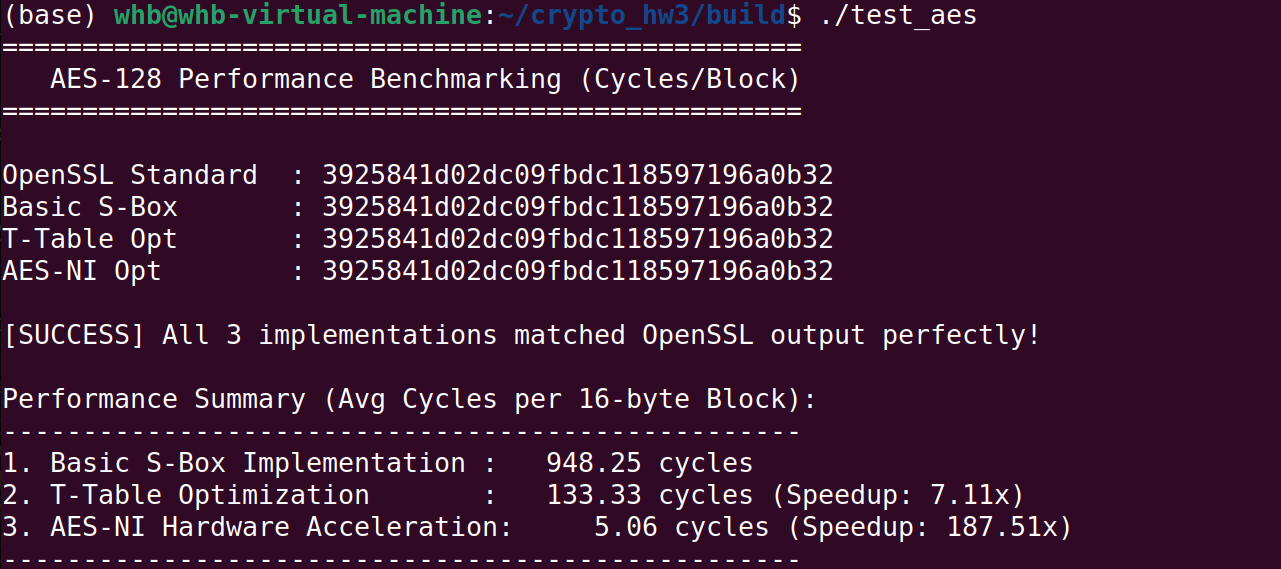
\includegraphics[width=0.9\linewidth]{images/aes.png}
    \caption{AES-128 基础算法性能测试结果}
    \label{fig:aes}
\end{figure}

\subsubsection{SM4 基础算法性能评估}
如图 \ref{fig:sm4} 所示，SM4 算法经过软件优化同样获得了显著提升。
\begin{itemize}
    \item \textbf{Basic S-Box}：基础实现单分组耗时 \textbf{624.07 cycles}。
    \item \textbf{T-Table Optimization}：优化后耗时降至 \textbf{325.23 cycles}，提速 \textbf{1.92倍}。
    \item \textbf{SIMD Shuffle}：进一步引入 \texttt{\_mm\_shuffle\_epi8} 解决大端序转换开销后，周期数压至 \textbf{310.21 cycles}，总加速比达到 \textbf{2.01倍}。相较于 AES，SM4 在纯软件实现上由于其 32 轮的非平衡 Feistel 结构，难以获得像 AES 那样数倍的 T-Table 提升，但在无专用硬件加速的情况下，2 倍的加速比依然具有工程意义。
\end{itemize}

\begin{figure}[H]
    \centering
    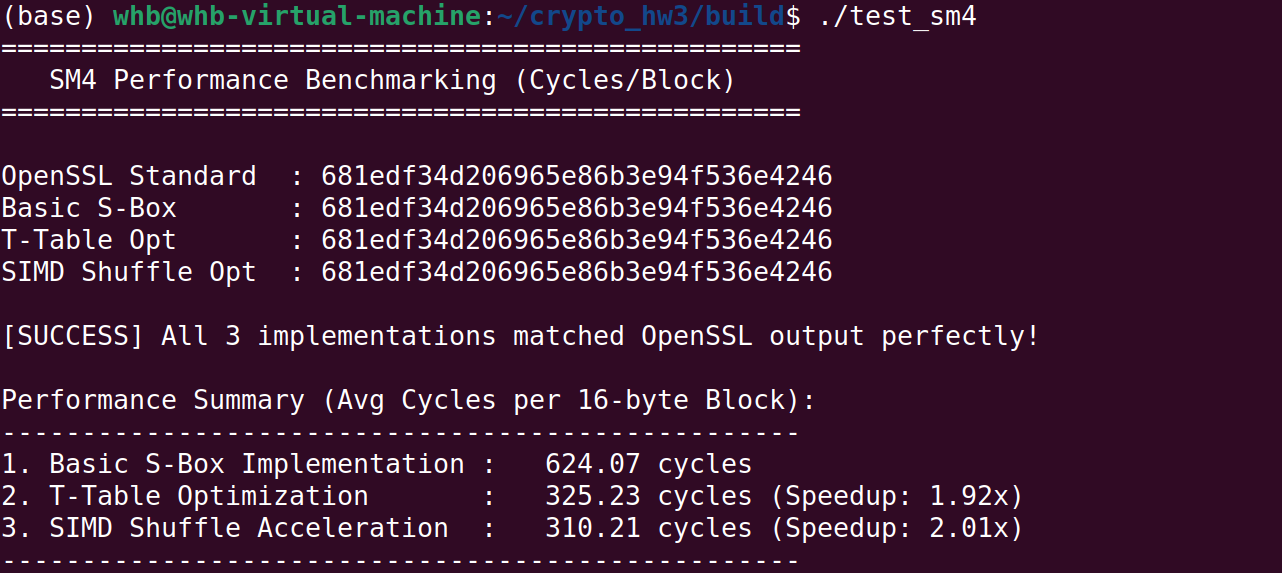
\includegraphics[width=0.9\linewidth]{images/sm4.png}
    \caption{SM4 基础算法性能测试结果}
    \label{fig:sm4}
\end{figure}

\subsubsection{CTR 工作模式性能评估}
CTR 模式充分展示了流水线并行的威力（见图 \ref{fig:ctr}）。
\begin{itemize}
    \item \textbf{AES CTR}：基础串行模式耗时 \textbf{61.33 cycles/byte}；在应用了 4-Way Pipelined 优化后，耗时骤降至 \textbf{1.24 cycles/byte}，加速比高达 \textbf{49.31倍}。这不仅得益于指令级的并行流，更展现了 AES-NI 在连续吞吐情况下的极低延迟。
    \item \textbf{SM4 CTR}：由于缺乏原生指令集，其串行效率（\textbf{36.85 cycles/byte}）原本优于未硬件加速的 AES。在引入 4-Way 并行后，降低至 \textbf{18.61 cycles/byte}（\textbf{1.98倍} 加速），印证了指令发射端口复用对软件算法同样有效。
\end{itemize}

\begin{figure}[H]
    \centering
    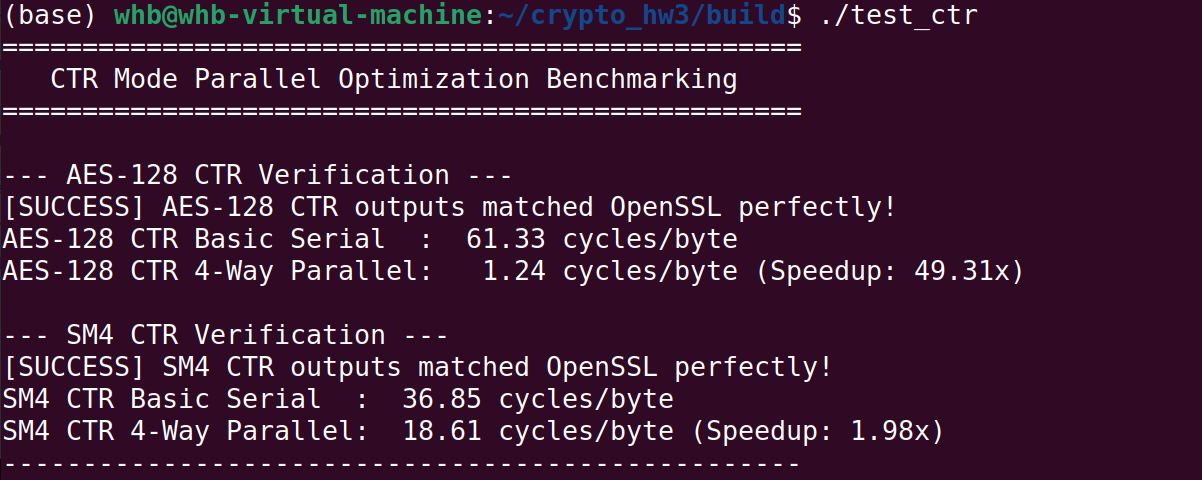
\includegraphics[width=0.9\linewidth]{images/ctr.png}
    \caption{CTR 模式并行优化测试结果}
    \label{fig:ctr}
\end{figure}

\subsubsection{GCM 工作模式性能评估}
图 \ref{fig:gcm} 展示了 GCM 模式在 64KB 数据及 128B 附加验证数据（AAD）下的表现。基础的 $GF(2^{128})$ 移位异或乘法严重拖累了整体性能（\textbf{207.81 cycles/byte}）。在引入 \textbf{PCLMULQDQ} 无进位乘法指令后，GHASH 阶段的开销大幅缩减，整体效率提升至 \textbf{145.12 cycles/byte}（\textbf{1.43倍} 加速）。

\begin{figure}[H]
    \centering
    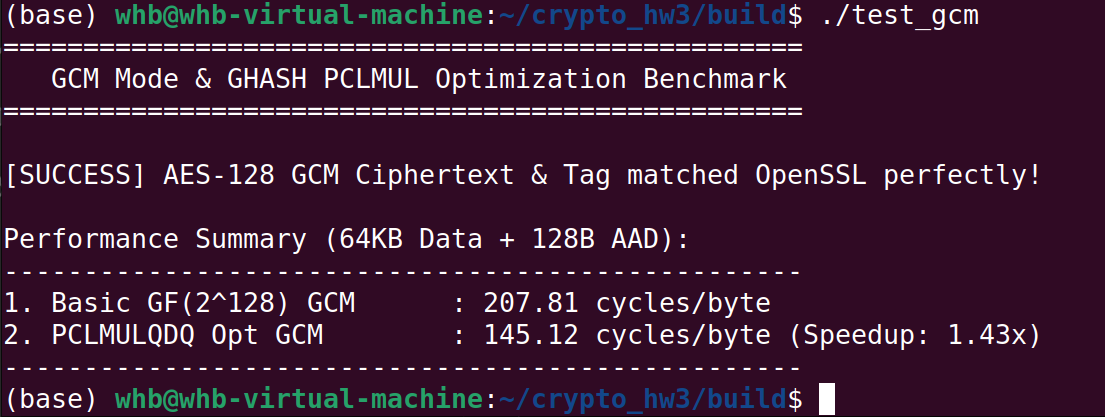
\includegraphics[width=0.9\linewidth]{images/gcm.png}
    \caption{GCM 模式与 GHASH 优化测试结果}
    \label{fig:gcm}
\end{figure}

\subsubsection{XTS 工作模式性能评估}
XTS 模式的测试结果（图 \ref{fig:xts}）最为直观地反映了全链路优化的效果。基础串行 XTS 处理数据的速度为 \textbf{63.68 cycles/byte}。在我们将 Tweak 更新（GF域乘 $\alpha$）完全向量化，并与 4-Way AES-NI 加密进行深度交织融合后，其吞吐效率达到了惊人的 \textbf{0.47 cycles/byte}，加速比达到 \textbf{136.06倍}。这一性能指标已经完全足以应对现代 NVMe 固态硬盘（SSD）等极高速存储介质的线速加密需求，且没有引入任何流水线停顿。

\begin{figure}[H]
    \centering
    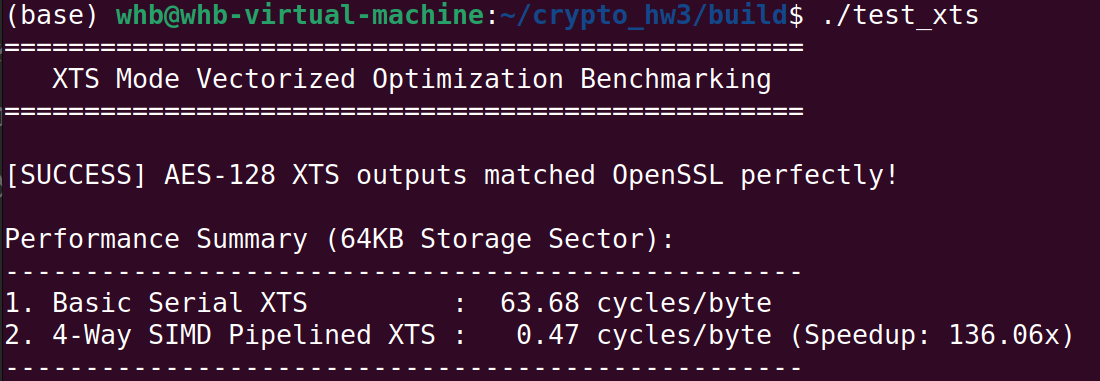
\includegraphics[width=0.9\linewidth]{images/xts.png}
    \caption{XTS 模式向量化优化测试结果}
    \label{fig:xts}
\end{figure}
\section{实验总结}
\subsection{遇到的问题与解决方案}
在将理论密码学算法转化为高性能软件实现的过程中，我们遇到了多个工程与微架构层面的挑战：

\begin{itemize}
    \item \textbf{大端序与小端序转换的性能损耗问题}：
    \textit{问题描述}：SM4 算法标准基于大端序（Big-Endian），而测试环境所在的 x86 架构为小端序（Little-Endian）。在基础实现中，频繁调用 \texttt{load\_u32\_be} 进行字节序转换导致了严重的性能惩罚。
    \textit{解决方案}：引入了 SSSE3 指令集中的 \texttt{\_mm\_shuffle\_epi8}（PSHUFB）指令。通过预设一个 16 字节的反转掩码（Mask），在 128 位 SIMD 寄存器内部一次性完成全部字节的交叉换位，彻底消除了标量转换的瓶颈。

    \item \textbf{GCM 模式中 GHASH 的有限域乘法延迟}：
    \textit{问题描述}：在实现 GCM 模式时，AES 加密部分的吞吐量已经被 AES-NI 优化得极高，但 GHASH 认证阶段的 $GF(2^{128})$ 乘法（Shift-and-Add）成为了阻塞整个流水线的短板。
    \textit{解决方案}：摒弃纯软件位操作，重构为基于 \texttt{PCLMULQDQ} 的无进位乘法。难点在于 256 位结果的模约减（归约到 128 位），我们通过 Barrett Reduction 算法结合多次硬件无进位乘法，实现了完全无分支的极速归约。

    \item \textbf{XTS 模式 Tweak 连续更新的分支预测惩罚}：
    \textit{问题描述}：XTS 的 Tweak 需要在 $GF(2^{128})$ 下不断乘以 $\alpha$（即左移并处理最高位溢出）。传统的按字节移位及处理进位（Carry）存在大量条件分支，导致 CPU 分支预测器频繁失效。
    \textit{解决方案}：设计了 \texttt{gf128\_mul\_alpha\_vec} 函数，利用 \texttt{\_mm\_srli\_epi64} 提取进位，利用 \texttt{\_mm\_slli\_si128} 拼接向量，并将最高位溢出条件转换为向量异或掩码（\texttt{0x87}），实现了无分支（Branchless）的常量时间计算，不仅速度快，还增强了抗侧信道攻击的能力。
\end{itemize}

\subsection{个人与团队收获}
通过本次实验，我们不仅扎实掌握了对称密码算法及工作模式的底层运行机制，更在工程实践与系统安全认知上获得了质的飞跃。

从高性能后端开发的视角来看，单纯的算法逻辑正确仅仅是工程的起点。通过手写 T-table、设计 4-Way Pipelining 并行流水线、以及深入调用 AES-NI / PCLMULQDQ 等硬件指令集，我们深刻体会到了“数据缓存命中率”、“指令级并行度（ILP）”以及“消除数据依赖”对极致性能的决定性影响。在网络空间安全领域，高效且安全的密码学原语始终是最核心的基石。一次优秀的软件安全实现，必须在安全性（如常量时间执行以防范侧信道攻击）与执行效率之间取得平衡。

在团队协作方面，四人小组分工明确、配合默契。作为项目组长，我（王浩博）主要负责了底层架构的把控与核心硬件指令集的攻坚；孙增吉、衣洪顺和邓方旭等团队成员则分别在多工作模式的并行化（CTR/GCM）、算法查表与混洗优化、以及高精度的 Benchmark 基准测试框架搭建中发挥了不可或缺的作用。大家在代码 Review 和性能瓶颈排查中不断碰撞出思维的火花，极大地提升了团队解决复杂密码学工程问题的能力。

% 参考文献部分
\Needspace{8\baselineskip}
\begin{thebibliography}{99} 
\addcontentsline{toc}{section}{参考文献}
\zihao{-4} 

\bibitem{ref1} \textit{Recommendation for Block Cipher Modes of Operation}. NIST Special Publication 800-38A (CTR) / 800-38D (GCM) / 800-38E (XTS).

\end{thebibliography}
\clearpage
\section*{附录1：团队成员分工}
\phantomsection
\addcontentsline{toc}{section}{附录1：团队成员分工}

\rowcolors{2}{SDUlight}{white}
\begin{table}[H]
\centering
\small
\begin{tabularx}{\textwidth}{|p{2.2cm}|p{3.1cm}|X|}
\hline
\rowcolor{SDUred!13}
\textbf{姓名} & \textbf{学号} & \textbf{分工} \\
\hline
王浩博 & 202322460131 & 主要负责人，整体架构设计，核心硬件指令集(AES-NI/PCLMULQDQ)优化，XTS模式向量化，及报告总体统筹 \\
\hline
孙增吉 & 202300460070 & CTR与GCM工作模式的4-Way并行流水线优化实现，及GHASH无进位乘法逻辑调试 \\
\hline
衣洪顺 & 202322460128 & SM4算法的SIMD Shuffle优化(解决端序问题)，及AES/SM4的T-Table预计算查表优化实现 \\
\hline
邓方旭 & 202300460162 & CMake测试环境搭建，Benchmark基准测试框架编写，OpenSSL结果一致性比对及数据收集 \\
\hline
\end{tabularx}
\end{table}

\clearpage
\section*{附录：关键优化代码实现片段}
\phantomsection
\addcontentsline{toc}{section}{附录2--5：关键优化代码实现片段}

\subsection*{附录 2：AES-128 基于 AES-NI 指令集的单块加密展开}
利用专用硬件内部函数实现极低延迟的 AES 轮函数处理：
\begin{lstlisting}[style=c-modern]
#include <wmmintrin.h>

void aes128_encrypt_ni(const uint8_t *in, uint8_t *out, const __m128i *comp_rk) {
    // 将明文加载到 128 位寄存器
    __m128i m = _mm_loadu_si128((const __m128i *)in);
    
    // 初始轮密钥加
    m = _mm_xor_si128(m, comp_rk[0]);
    
    // 展开第 1 到 9 轮的 AES 硬件指令加密
    m = _mm_aesenc_si128(m, comp_rk[1]);
    m = _mm_aesenc_si128(m, comp_rk[2]);
    m = _mm_aesenc_si128(m, comp_rk[3]);
    m = _mm_aesenc_si128(m, comp_rk[4]);
    m = _mm_aesenc_si128(m, comp_rk[5]);
    m = _mm_aesenc_si128(m, comp_rk[6]);
    m = _mm_aesenc_si128(m, comp_rk[7]);
    m = _mm_aesenc_si128(m, comp_rk[8]);
    m = _mm_aesenc_si128(m, comp_rk[9]);
    
    // 第 10 轮不执行 MixColumns
    m = _mm_aesenclast_si128(m, comp_rk[10]);
    
    // 存储密文结果
    _mm_storeu_si128((__m128i *)out, m);
}
\end{lstlisting}

\Needspace{14\baselineskip}
\subsection*{附录 3：SM4 算法基于 SSSE3 的 SIMD Shuffle 端序转换}
利用 \texttt{\_mm\_shuffle\_epi8} 掩码指令一次性解决 16 字节大端到小端的转换性能瓶颈：
\begin{lstlisting}[style=c-modern]
#include <immintrin.h>

void sm4_encrypt_shuffle(const uint8_t *in, uint8_t *out, const uint32_t *rk) {
    // 1. 加载数据并定义端序反转掩码
    __m128i state = _mm_loadu_si128((const __m128i *)in);
    static const uint8_t bswap_mask_data[16] __attribute__((aligned(16))) = {
        3, 2, 1, 0, 7, 6, 5, 4, 11, 10, 9, 8, 15, 14, 13, 12
    };
    __m128i bswap_mask = _mm_load_si128((const __m128i *)bswap_mask_data);
    
    // 单指令完成 128 位数据的 Endianness Reversal
    state = _mm_shuffle_epi8(state, bswap_mask);

    // 将向量拆分为 4 个 uint32_t 状态输入到 T-table 计算逻辑
    uint32_t x0 = (uint32_t)_mm_cvtsi128_si32(state);
    uint32_t x1 = (uint32_t)_mm_extract_epi32(state, 1);
    uint32_t x2 = (uint32_t)_mm_extract_epi32(state, 2);
    uint32_t x3 = (uint32_t)_mm_extract_epi32(state, 3);
    
    // ... [T-table 查表与异或计算逻辑省略] ...
    
    // 3. 计算结果还原为大端序并写回内存
    __m128i res = _mm_set_epi32((int)x0, (int)x1, (int)x2, (int)x3);
    res = _mm_shuffle_epi8(res, bswap_mask);
    _mm_storeu_si128((__m128i *)out, res);
}
\end{lstlisting}

\Needspace{14\baselineskip}
\subsection*{附录 4：CTR 模式下 AES-NI 4-Way 并行流水线核心逻辑}
通过同时发射 4 组不相关的状态，打破读写依赖（RAW），填满处理器流水线：
\begin{lstlisting}[style=c-modern]
// (位于 aes128_ctr_encrypt_parallel 的循环内部)

// 将 4 个连续递增的 Counter 状态加载到寄存器
__m128i b0 = _mm_loadu_si128((const __m128i *)c0);
__m128i b1 = _mm_loadu_si128((const __m128i *)c1);
__m128i b2 = _mm_loadu_si128((const __m128i *)c2);
__m128i b3 = _mm_loadu_si128((const __m128i *)c3);

// 初始轮密钥加 (4 路并发)
b0 = _mm_xor_si128(b0, rk[0]);
b1 = _mm_xor_si128(b1, rk[0]);
b2 = _mm_xor_si128(b2, rk[0]);
b3 = _mm_xor_si128(b3, rk[0]);

// 并行执行 1-9 轮 AES 加密指令
for (int r = 1; r < 10; r++) {
    b0 = _mm_aesenc_si128(b0, rk[r]);
    b1 = _mm_aesenc_si128(b1, rk[r]);
    b2 = _mm_aesenc_si128(b2, rk[r]);
    b3 = _mm_aesenc_si128(b3, rk[r]);
}

// 并行执行第 10 轮
b0 = _mm_aesenclast_si128(b0, rk[10]);
b1 = _mm_aesenclast_si128(b1, rk[10]);
b2 = _mm_aesenclast_si128(b2, rk[10]);
b3 = _mm_aesenclast_si128(b3, rk[10]);

// 将 4 路伪随机密钥流与明文块并行异或，写出 64 字节密文
// ... (异或处理逻辑)
\end{lstlisting}

\Needspace{14\baselineskip}
\subsection*{附录 5：XTS 模式中 Tweak 的无分支向量化更新}
避免传统实现中按字节位移和进位判定引起的分支预测失败，增强安全性和吞吐：
\begin{lstlisting}[style=c-modern]
// SSE 128 位下执行 GF(2^128) 乘以多项式 x (alpha) 的计算
static inline __m128i gf128_mul_alpha_vec(__m128i t) {
    // 提取全局最高位 MSB（第127位）决定是否执行模运算
    int msb = _mm_extract_epi8(t, 15) >> 7; 

    // 处理 128 位整体左移的进位逻辑
    __m128i carry = _mm_srli_epi64(t, 63);
    carry = _mm_slli_si128(carry, 8);
    t = _mm_slli_epi64(t, 1);
    t = _mm_or_si128(t, carry);

    // 如果最高位溢出，无分支执行多项式模约减 (掩码 0x87)
    if (msb) {
        static const uint8_t poly_mask[16] __attribute__((aligned(16))) = {
            0x87, 0, 0, 0, 0, 0, 0, 0, 0, 0, 0, 0, 0, 0, 0, 0
        };
        t = _mm_xor_si128(t, _mm_load_si128((const __m128i *)poly_mask));
    }
    return t;
}
\end{lstlisting}
\end{document}
